\chapter{Algorithm configuration}
\label{ch:Algorithm configuration}
Many of the methods proposed in chapter \ref{ch:Analysis of the pattern recognition problem} require hyper-parameters that vary aspects of the algorithm and might lead to better or worse results. To ensure that all the algorithms are comparable with each other this chapter goes over the process of finding the optimal hyper-parameters for every approach. A comparable score is assigned to every algorithm under the condition of optimal hyper-parameters.
\section*{Hyper-parameter tuning}
The process of searching and finding good hyper-parameters for a given algorithm is called hyper-parameter tuning. Searching for good hyper parameters takes the following aspects to be considered:
\begin{itemize}
\item{ \textbf{an estimator}} \\
The estimator in this case is a binary classifier. The 8 different binary classifiers have to be considered as mentioned in chapter \ref{ch:Analysis of the pattern recognition problem}.
\item{\textbf{a parameter space}} \\
The parameter space defines a set of parameters or combination of parameters that will be tested. From this set one element will be chosen as most fitting. Because every algorithm requires different parameters, the parameter space is different for every algorithm. The parameter space will be defined in the sections below for every algorithm. 
\item{\textbf{a method for searching or sampling candidates}}\\
The method that is chosen is grid search. Grid search is a brute force search, which uses an exhaustive searching through a defined parameter space. Models and iteratively trained and evaluated by a score function. The model scores are then compared. The hyper-parameters that produced the best performing model will be chosen as optimal ones for the algorithm.
\item{\textbf{a cross-validation scheme}} \\
The cross-validation scheme used is a k-fold validation, with k=10.
\item{\textbf{a score function}}\\
As mentioned in chapter \ref{ch:Analysis of the pattern recognition problem}  a  f\textsubscript{2}-score will be used to evaluate the models in the end. Our goal for the hyper-parameter tuning is thereby also to maximise the  f\textsubscript{2}-score. For that reason the  f\textsubscript{2}-score is used as a score function.
\end{itemize}

For the hyper-parameter search no external functions or libraries are used. The search algorithm is implemented in the following way.\\ For a given estimator (in this case one of the possible classification algorithms) the parameter space is defined manually for every hyper-parameter of a given estimator.\\
Models are now repeatedly trained by iterating through every combination of hyper-parameters in the parameter spaces.\\
For every trained model a  k-fold validation, with k=10, is performed.\\
During the k-fold validation, the f\textsubscript{2}-score is calculated.\\
After this process is done the hyper-parameters that resulted in the highest f\textsubscript{2}-score are chosen.\\
For the each of the relevant algorithms a parameter space will be defined. The results of the hyper parameter search will then be presented.

\subsection*{Linear SVM}
\subsection*{Logistic regression}
\subsection*{Decision tree}
The tunable hyper-parameters for the decision tree algorithm are:
\begin{itemize}
\item{\textbf{Impurity}}\\
The impurity measure is used to decide on a splitting rule for each node in the decision tree building process.
Two impurity measures for classification are provided:\\
\textbf{Gini impurity:}  \\
$\sum_{i=1}^{C} f\textsubscript{i}(1-f\textsubscript{i}) $ \\
C is the number of unique labels and f\textsubscript{i} is the frequency of label i in a node. \\
\textbf{Entropy:}\\
$\frac{1}{N}\sum_{i=1}^{C} -f\textsubscript{i}\log(f\textsubscript{i}) $ \\
C is the number of unique labels and f\textsubscript{i} is the frequency of label i in a node. \\
\item{\textbf{Maximal depth}}\\
The maximal depth determines a limit of growth for a decision tree. This consequentially limits the number of nodes or decisions that are possible. It represents a stopping criteria. \\
The parameter space for the maximal depth is chosen \textbf{from 1 to 10} (inclusive). 
\end{itemize}

The hyper-parameter search reveals the following results: \\

\pgfplotsset{width=1.1\textwidth, height=0.5\textwidth}

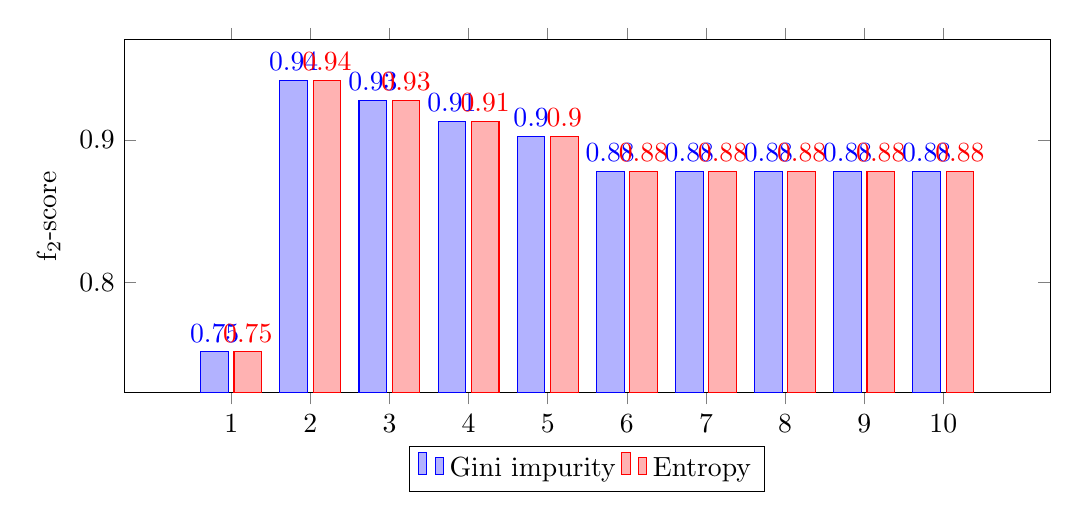
\begin{tikzpicture}
\begin{axis}[
ybar,
enlargelimits=0.15,
legend style={at={(0.5,-0.15)},
anchor=north,legend columns=-1},
xlabel={Maximal depth},
ylabel={f\textsubscript{2}-score},
symbolic x coords={1,2,3,4,5,6,7,8,9,10},
xtick=data,
nodes near coords,
nodes near coords align={vertical},
]
\addplot coordinates {(1, 0.7514765369250439)	(2, 0.94167516977742205)	(3, 0.92745939539660371)	(4, 0.91277351764611503)	(5, 0.90267105713062501)	(6, 0.87786051720271308)	(7, 0.87786051720271308)	(8, 0.87786051720271308)	(9, 0.87786051720271308)	(10, 0.87786051720271308)
};

\addplot coordinates {(1, 0.7514765369250439)	(2, 0.94167516977742205)	(3, 0.92745939539660371)	(4, 0.91277351764611503)	(5, 0.90267105713062501)	(6, 0.87786051720271308)	(7, 0.87786051720271308)	(8, 0.87786051720271308)	(9, 0.87786051720271308)	(10, 0.87786051720271308)
};
\legend{Gini impurity,Entropy}
\end{axis} 
\end{tikzpicture}
\\
The best performing decision tree model reaches a maximal {f\textsubscript{2}-score of \textbf{0.94} (precision:  0.92, recall: 0.96) with the following hyper-parameters:\\
Impurity: \qquad  \qquad \textbf{Ginni Impurity} or \textbf{Entropy} \\
Maximal depth: \qquad \textbf{2}




\subsection*{Random forest}
\subsection*{Gradient-boosted trees}
\subsection*{Naive Bayes}
 